\chapter{Einleitung}

Im folgenden Abschnitt werden die aus technischer Sicht relevanten Aspekte genauer analysiert. Zu Beginn wird das Aufgabenumfeld in einem weiteren Sinne betrachtet, und die Kernelemente der Applikation aufgezeigt. Danach wird auf die Analyse und die Realisierung eingegangen.
\\
Der Hauptteil richtet sich vor allem an Personen, die bereits Hintergrundwissen zu Android vorweisen, sowie für Entwickler, die an der Weiterentwicklung des Produktes interessiert sind.

\section{BigPicture}
Zur Übersicht wird das Umfeld der Applikation in einem BigPicture zusammengefasst. Es ermöglicht die Darstellung der äusseren Einflussfaktoren sowie die Abgrenzung des Systems zu definieren.
\\
Die schematische Darstellung zeigt im wesentlichen die drei Hauptakteure auf. Zum einen sind dies die Motorradfahrer, welche die Radrennfahrer begleiten und Veränderungen in Echtzeit per Funk übermitteln. Diese Informationen kommen in kurzen Abständen und müssen sofort erfasst werden. Im UserInterface wird dafür eine Lösung verwendet, bei der mehrere Radrennfahrer gleichzeitig eingetragen werden können.
\\
Eine weitere Rolle spielt der \textit{RadioTour Speaker} mit dem Android Tablet. Er fasst die Informationen zusammen und wertet diese bereits bei der Eingabe auf dem Gerät aus. Im Tablet werden auch Daten wie z.B. die Durchschnittsgeschwindigkeit und die aktuelle Rennzeit angezeigt.
\\
Der dritte Akteur bildet der Server der cnlab AG, welcher direkt mit der Applikation kommuniziert. Ausgetauscht werden die Veränderungen im Feld sowie Rückstände von der Spitze. Weiter können Ereignisse wie z.B. eine Verletzung oder ein defektes Fahrrad aufgezeichnet werden. Die Daten werden dann weiter auf der Webseite der \textit{TourLive} aufbereitet und publiziert. Nicht nur für die Beteiligten im Team, sondern auch für Fans sind diese Angaben von grossem Interesse, da die Daten vor den offiziellen Zeitmessungen bereits einen Einblick in das Schlussklassement geben.

\newpage

\begin{figure}[h!]
\caption{Das Aufgabenumfeld in einem BigPicture zusammengefasst}
\centering
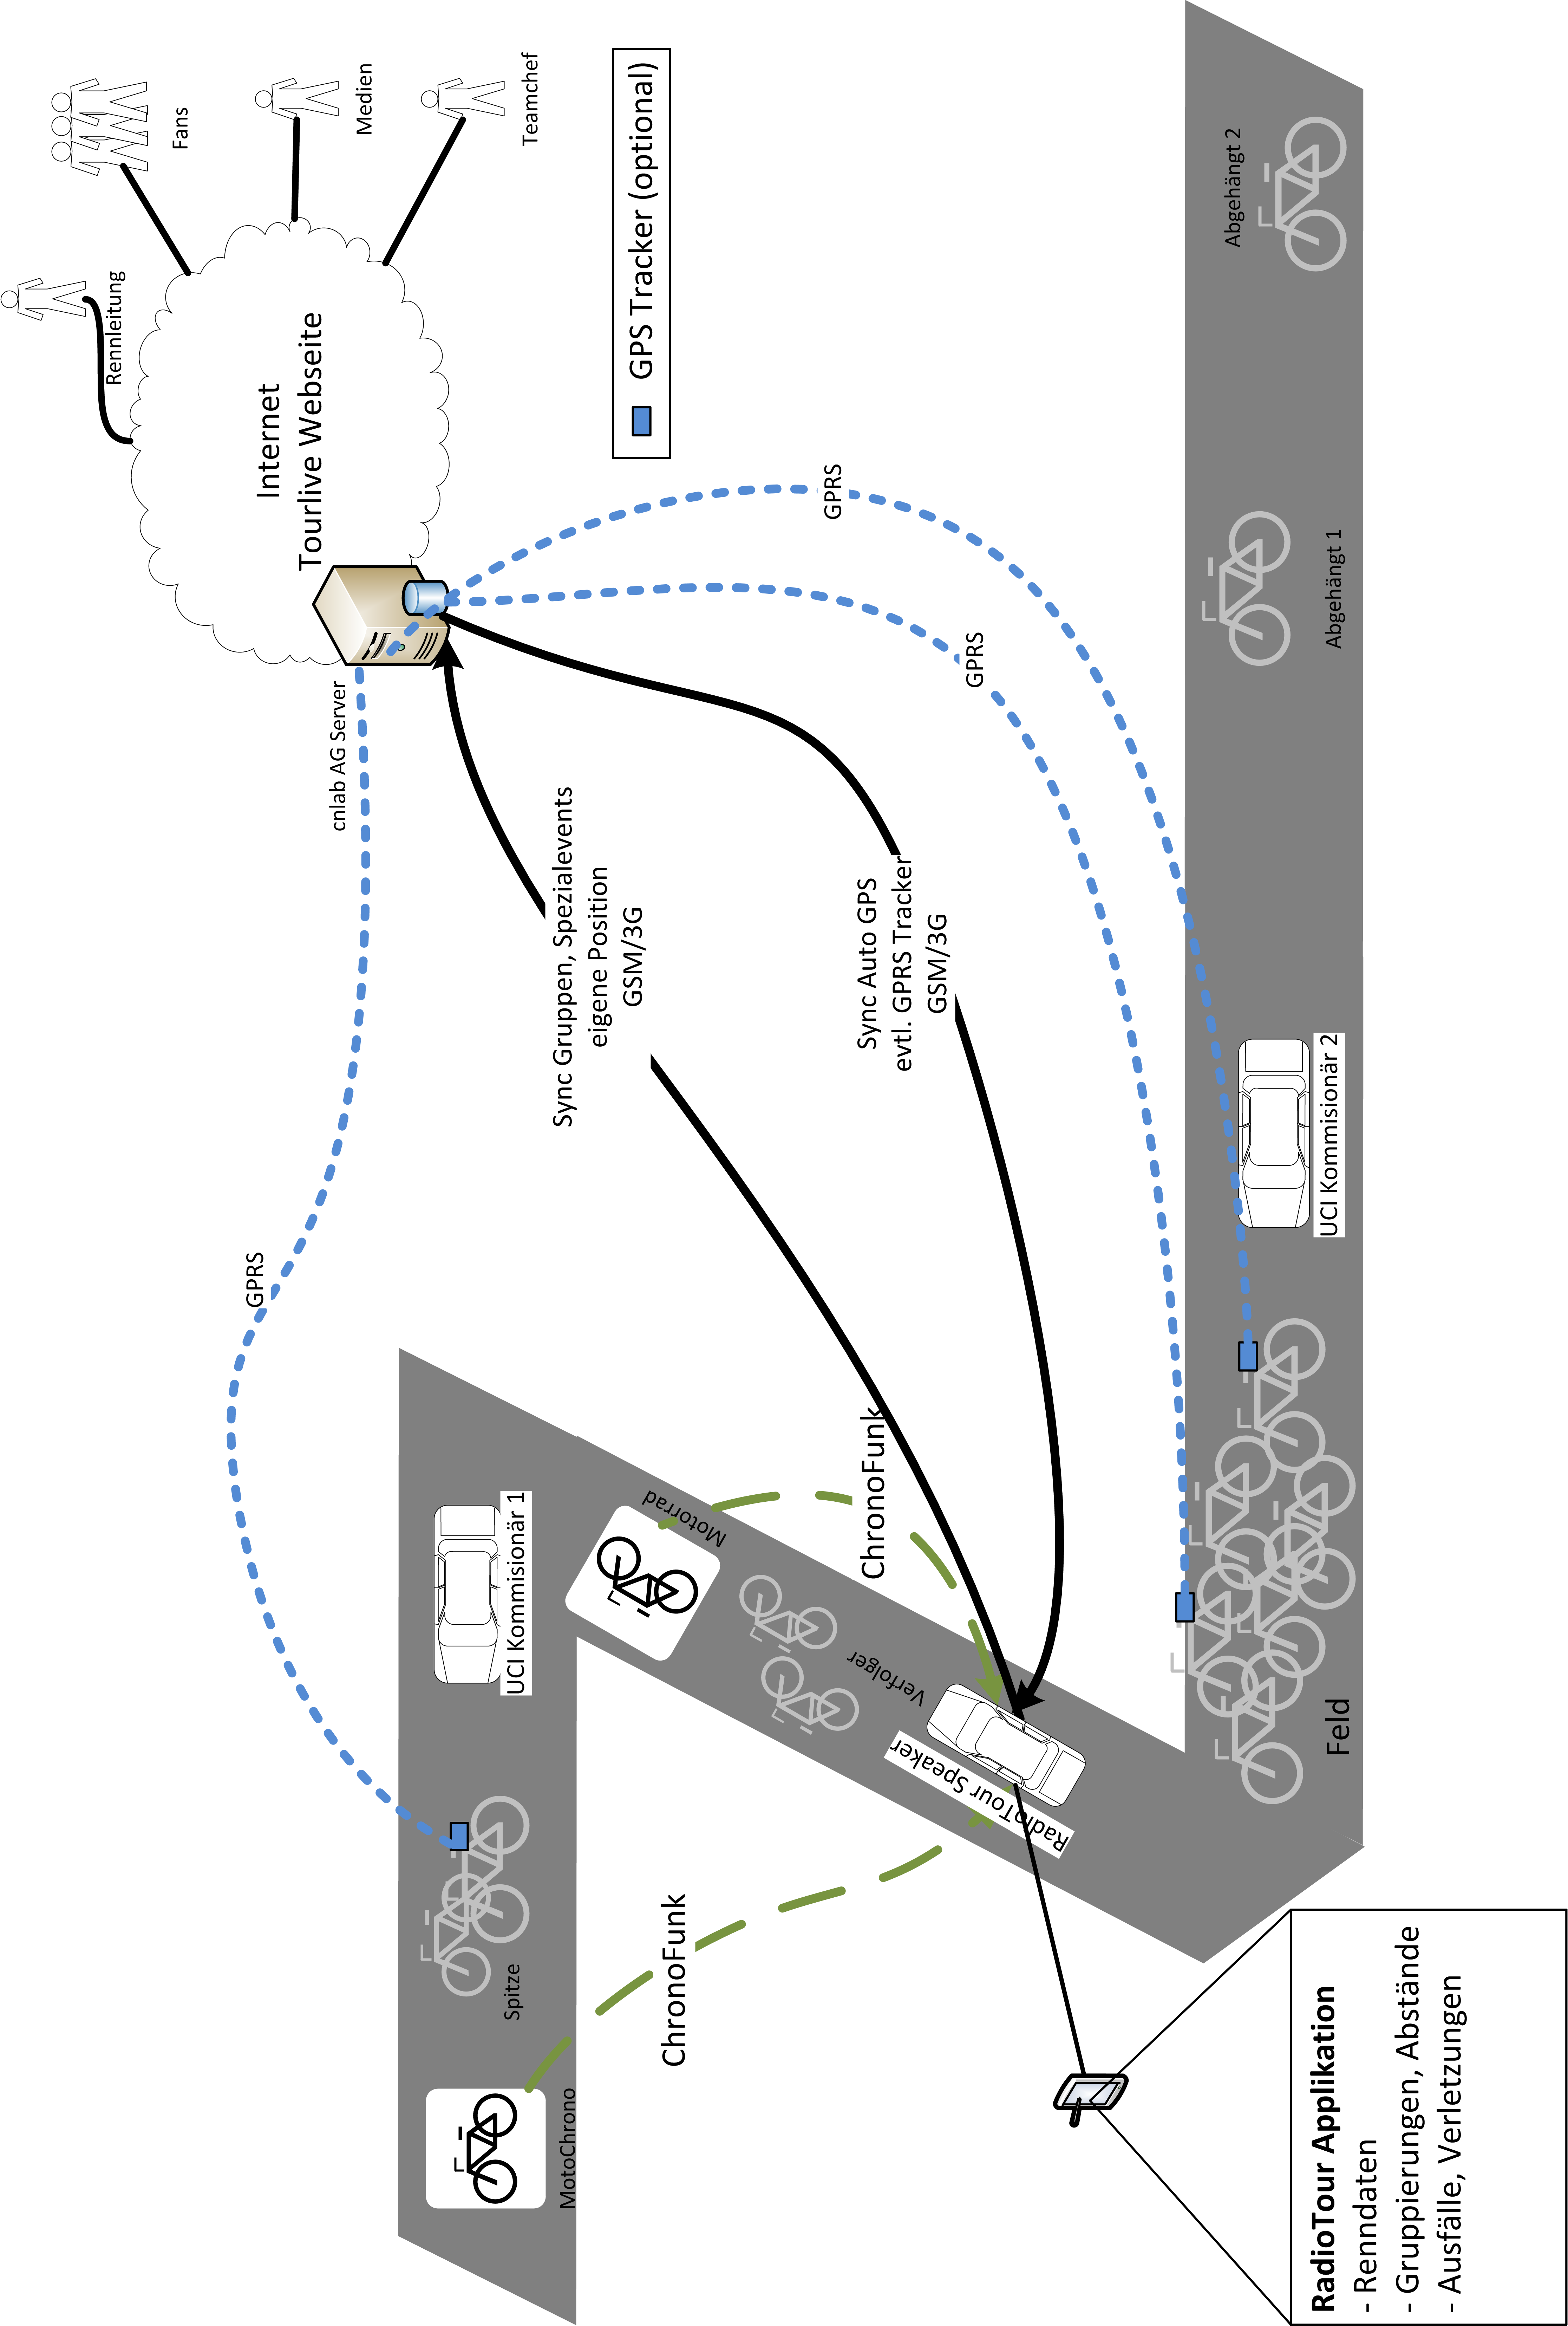
\includegraphics[scale=0.7]{05bericht/images/bigpicture.png}
\end{figure}

\newpage

\section{Kernelemente}
Das Produkt dieser Arbeit ist es, die Tabletanwendung für den \textit{RadioTour Speaker} zu entwickeln. Der Hauptfokus liegt dabei auf der Erfassung der Rennsituation und die sichere Übertragung an den Server. In der Abbildung \ref{fig:closepicture} steht die Applikation im Mittelpunkt und zeigt die \gls{http} Schnittstelle zum TourLive Server. Die Positionsdaten werden von den GPS Satelliten empfangen und die Datenpersistierung basiert auf einer \gls{sqlite} Datenbank. In der Applikation ist die Hauptansicht für die Situation während einem Rennen zu sehen.
\\

\begin{figure}[h!]
\caption{Die genaue Betrachtung der Aufgaben der Applikation}
\label{fig:closepicture}
\centering
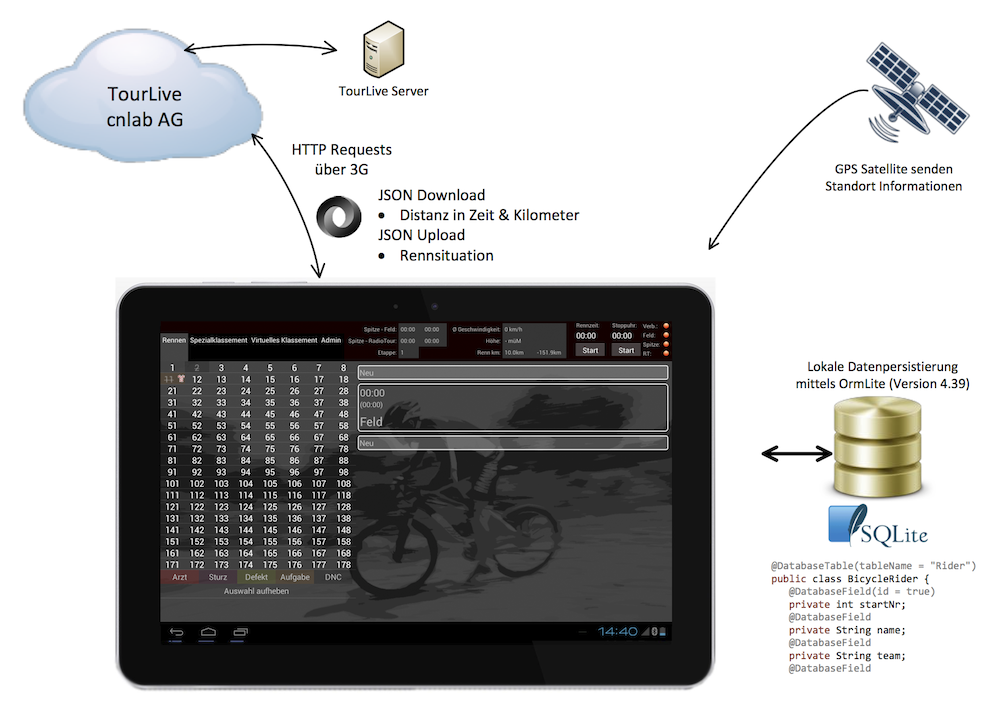
\includegraphics[scale=0.8]{05bericht/images/closepicture.png}
\end{figure}
